\chapter{Materials \& Methods}
\section{Overview}

In this section, an overview of the system architecture for the emotion recognition system developed for a resource-limited robotic platform is presented. The architectural diagram (see \ref{figure:architecturediagram}) illustrates how data flows from sensor acquisition through processing to decision-making, enabling the robot to determine human emotional states in real time. The system is composed of two primary modules: the image-based emotion recognition module and the speech-based emotion recognition module, each designed to operate independently while allowing the system to select the most appropriate modality based on contextual demands.

The image-based module begins with the acquisition of visual input via a camera. This input is processed through a face detection component where three methods---Haar Cascades, Dlib HOG+SVM, and YOLOv4---are implemented and compared to determine the most effective approach for isolating faces under varying conditions. Once faces are detected, the resulting regions of interest are forwarded to an emotion classification sub-module. Here, several convolutional neural network (CNN) architectures, including VGG16, ResNet50, and MobileNetV2, are evaluated for their ability to classify the emotional expressions accurately. The CNN models are trained using transfer learning on a dataset of labelled facial images representing seven basic emotions: happiness, sadness, anger, surprise, fear, disgust and contempt. The trained models are then deployed on the robot to process real-time video streams and classify the emotions of human subjects.

Concurrently, the speech-based module captures auditory input through an onboard microphone. This audio stream is first transcribed into text by the \texttt{speech\_recognition} Python library. The transcribed text is then analysed for emotional content using sentiment analysis provided by IBM Watson Cloud Services. By processing these two streams separately, the system can dynamically choose between visual and auditory modalities, ensuring that the most reliable source of emotion data is used based on the situational context.

\begin{figure}[!htb]
    \centering{}
    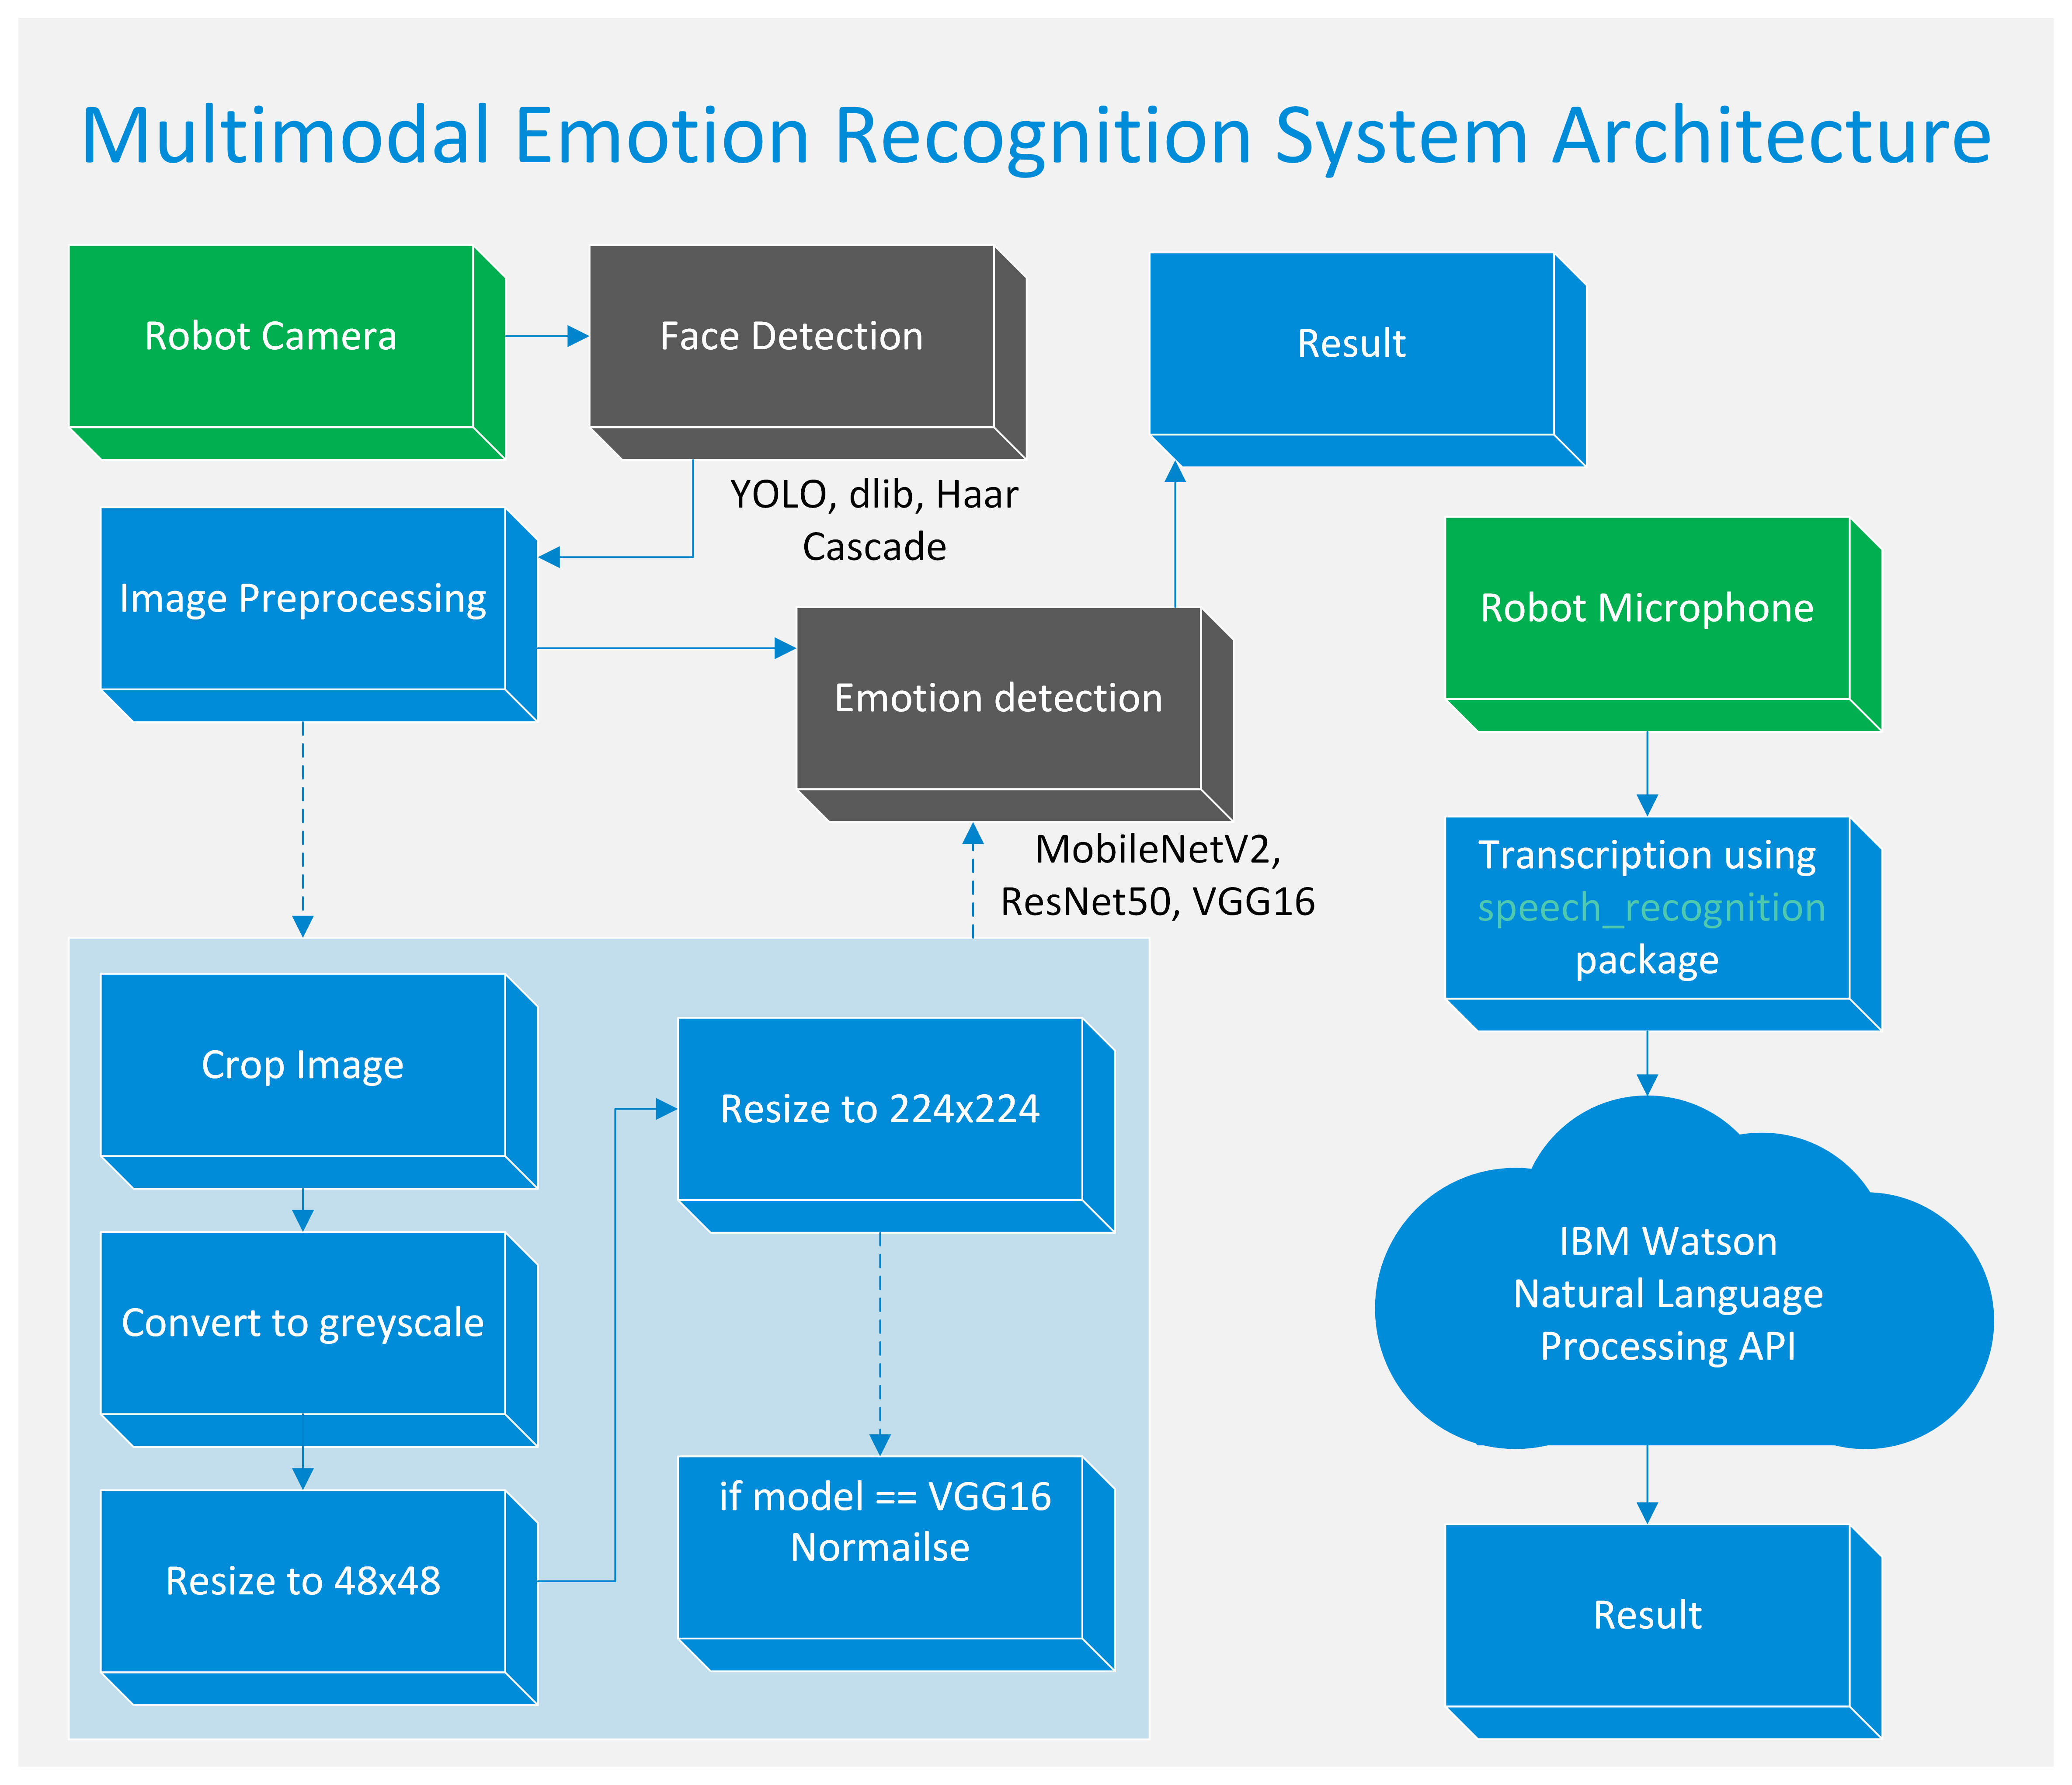
\includegraphics[scale=0.35]{m+m_images/ArchitectureDiagram.png}
    \caption{Architecture diagram showing the integration of facial and sentiment analysis components}
    \label{figure:architecturediagram}
\end{figure}

The development process was iterative, beginning with the independent design and validation of each module using established datasets for face detection and visual emotion classification. Following individual validation, the modules were integrated into a unified framework capable of processing real-time data from the robot's sensors. Rigorous testing was conducted using annotated datasets designed to simulate real-world conditions to assess the system's accuracy, processing speed, and overall resource utilisation.

Overall, the architectural design emphasises modularity and flexibility, allowing for individual components to be updated or replaced without impacting the entire system. This design not only streamlines development and testing but also positions the system for future enhancements and adaptations as the requirements of human-robot interaction evolve.

\section{Materials}

\subsection{Robot Platform}

The TurtleBot 4 is a sophisticated and versatile robotic platform designed for research, education, and experimentation in the fields of robotics and artificial intelligence (AI). It is an evolution of the TurtleBot series, integrating advanced hardware and software components to provide enhanced functionality and performance.

\subsubsection{Hardware Components}
The Turtlebot4 is equipped with an iRobot® Create3 mobile base, based on the Roomba®, a robot vacuum cleaner. At the front of the robot is a multizone bumper equipped with seven sets of IR proximity sensors, allowing for seamless obstacle detection. The OAK-D spatial AI stereo camera enables the robot to perceive the world in a human-like manner by combining a stereo depth camera and a high-resolution colour camera with on-device Neural Network inferencing and Computer Vision capabilities.

\begin{figure}[!htb]
    \centering{}
    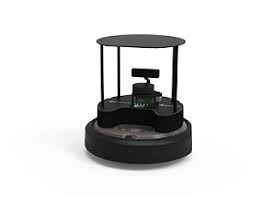
\includegraphics[scale=0.5]{m+m_images/tb4.jpg}
    \caption{Turtlebot 4}
    \label{figure:tb4}
\end{figure}


The robot features a Raspberry PI 4 equipped with Broadcom BCM2711, Quad-core Cortex-A72 (ARM v8) 64-bit SoC running at 1.8GHz and XGB of LPDDR4-3200 SDRAM.

The robot uses a standard Lithium Ion Battery designed for Roomba® e \& i series robots. The battery onboard with the robot is a 26 Wh, 4S Lithium-Ion smart battery pack, with a nominal voltage of 14.4 V (12 V min, 16.8 V max).

The TurtleBot 4 is built on ROS, a flexible framework for developing robotic applications. ROS provides a set of tools and libraries for various tasks such as sensor data processing, navigation, and control. The TurtleBot 4, specifically, comes equipped with ROS2 Humble with the Raspberry PI 4 running on Ubuntu 22.04.

\subsection{Training Computer}

Since training efficiency is not the focus of this project, the HP Z8 G4 Workstation is its training PC, a high-performance computing solution tailored for intensive professional tasks. The system features dual Intel Xeon Gold 6244 CPUs with 8 cores and 16 threads operating at 3.60GHz, 512 GB of Samsung ECC RAM running at 2666MT/s, and two NVIDIA Quadro RTX 8000 GPUs with 48GB of GDDR6 memory each.

The development environment was set up using Python 3.10.12 on the training PC with Ubuntu 22.04. Image processing and face detection were handled using OpenCV 4.5, the Dlib library and darknet by Alexeyab \cite{Alexey_2021-lf}. TensorFlow 2.15.1 and Keras were used to develop and train CNN models. Speech analysis was performed using the IBM Watson Speech-to-Text API.

\section{Methods}

To implement emotion detection algorithms, we will utilise various software libraries and frameworks tailored to different aspects of the task. This section outlines the methodologies and tools that will be employed for both facial detection and emotion recognition.
\subsection{Facial Detection Algorithms}

\subsubsection{Haar Cascade}

The emotion recognition system considers the Haar Cascade model as a choice for face detection. This pretrained model is easily accessible and adept at identifying faces in images. The Haar Cascade algorithm, created by Viola and Jones \cite{Viola990517}, is a well-regarded technique for object detection, with a particular emphasis on detecting faces within images.

The Haar Cascade algorithm identifies a collection of rectangular features referred to as Haar-like features. These features are basic designs that exhibit variations in pixel intensities across adjacent sections of the image. To efficiently compute these Haar-like features, the algorithm leverages an integral image representation of the input image. The integral image enables swift computation of the total sum of pixel intensities within any given rectangular area of the image.
The following step entails instructing a series of weak classifiers with the Adaboost learning algorithm. Each of these classifiers is taught to recognise a particular Haar-like feature that is indicative of the intended object, such as a face. Throughout the training process, Adaboost allocates greater importance to incorrectly classified examples, directing subsequent iterations towards rectifying these mistakes.
\begin{figure}[!htb]
    \centering{}
    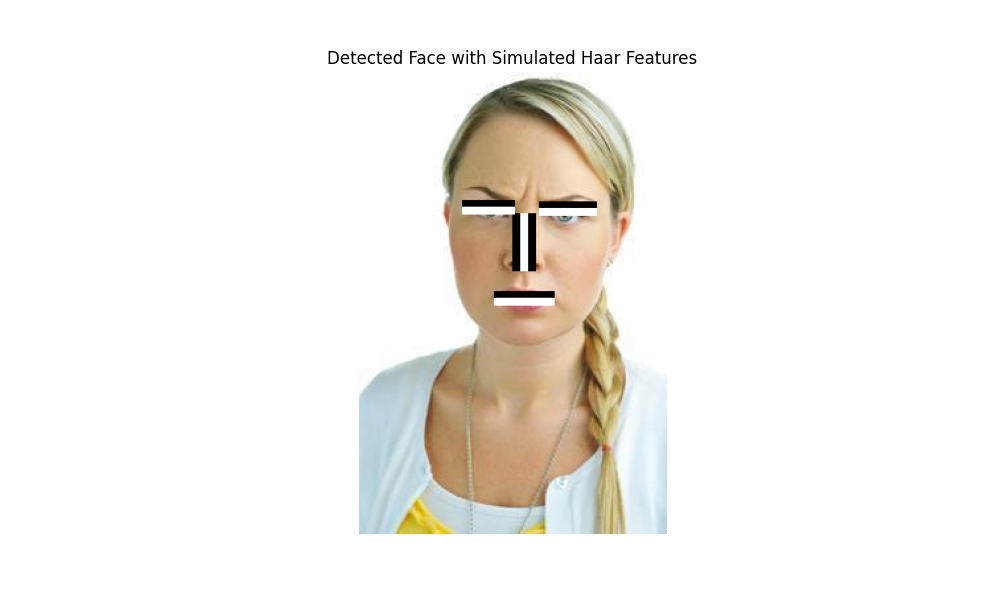
\includegraphics[scale=0.5]{m+m_images/HaarFeatures.png}
    \caption{Image showing Haar-like features used in the Haar Cascade algorithm}
    \label{figure:haarfeature}
\end{figure}

The Haar Cascade classifier utilises a cascade structure to organise trained weak classifiers. Sequentially arranged, each stage of the cascade consists of multiple weak classifiers. The cascade design enables early stages to swiftly reject negative examples, while positive examples proceed to subsequent stages for further evaluation. During the detection phase, the Haar Cascade algorithm utilises a sliding window approach to scan the input image. At each position of the sliding window, the algorithm applies each stage of the cascade sequentially, rapidly discarding regions of the image that are unlikely to contain the target object based on the results of earlier stages.

\begin{figure}[!htb]
    \centering{}
    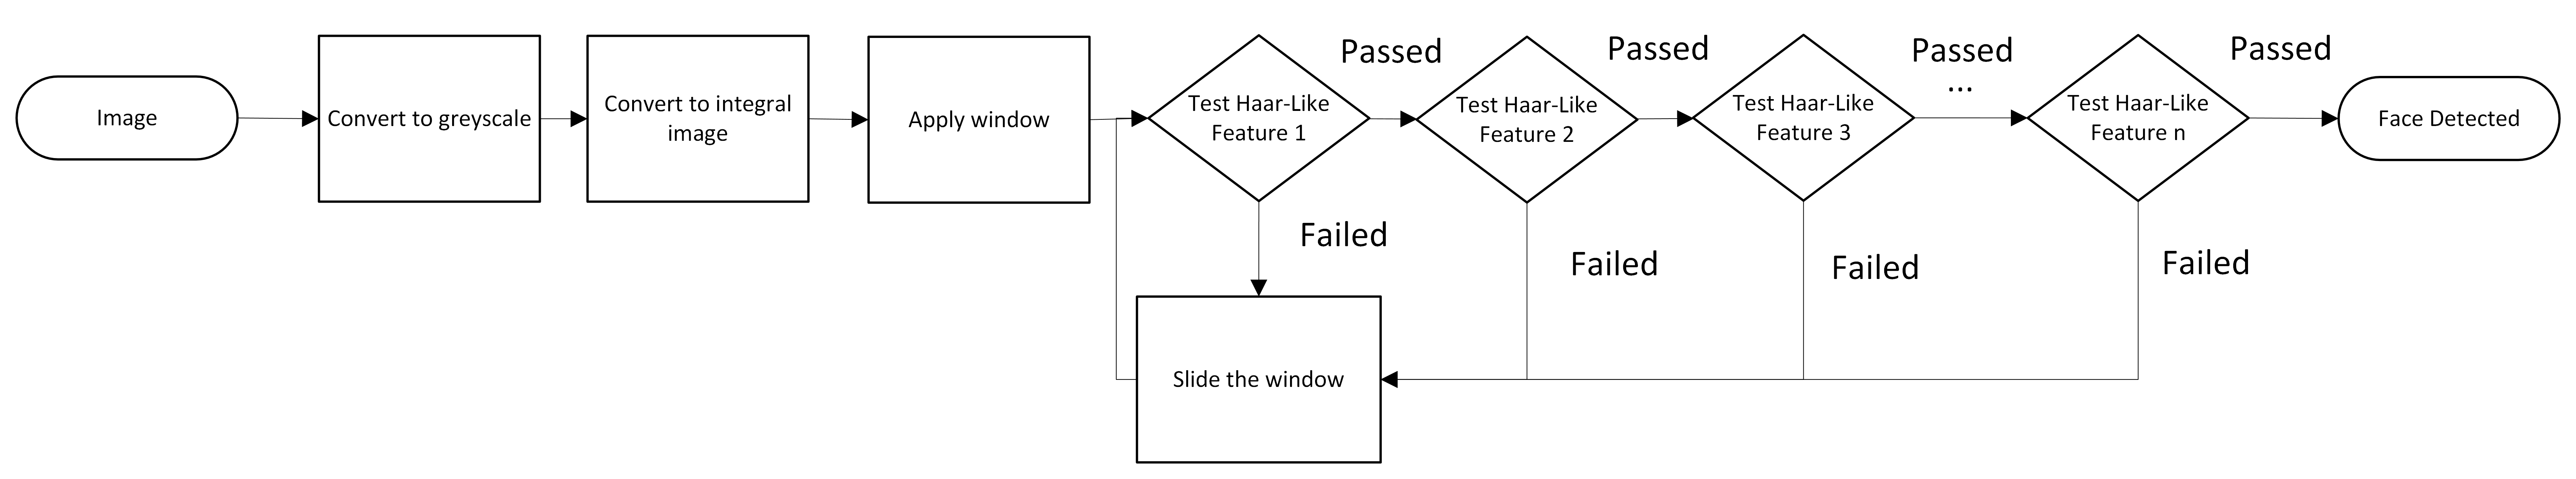
\includegraphics[scale=0.25]{m+m_images/HaarCascadeDesign.png}
    \caption{Image showing how the Haar Cascade algorithm rapidly discards regions of the image that are unlikely to contain the target object}
    \label{figure:haardesign}
\end{figure}

After going through all the stages of the cascade, the regions of the image that meet the criteria for the target object are identified as positive detections. The algorithm provides the location and size of the detected objects in the image by producing bounding boxes around these regions.

One of the key advantages of the Haar Cascade model is its efficiency and ease of implementation. It is pre-trained on an extensive dataset of labeled face images, allowing for immediate use without the need for additional training. The training set comprises 4,916 hand-labeled faces, all scaled and aligned to a base resolution of 24\(\times\)24 pixels, ensuring consistency and accuracy in detection. These faces were extracted from a diverse set of images collected through a random crawl of the World Wide Web, offering robustness across various scenarios. Additionally, the model is evaluated on the MIT+CMU test set, which includes 130 images and 507 faces, demonstrating its capability to perform well even in complex, real-world conditions. Notably, Haar Cascade is renowned for its computational efficiency, making it ideal for real-time applications, especially in resource-constrained environments where rapid face detection is crucial.

\subsubsection{YOLO}

The You Only Look Once (YOLO) model for object detection is a highly efficient and accurate approach for real-time object detection in images and videos. This model is known for its unique architecture and approach, which enable it to detect objects with remarkable accuracy. The YOLO model has gained popularity in the academic and research communities due to its exceptional performance, and it has become an important tool for various applications in computer vision and machine learning.

YOLO's heart lies its single neural network architecture that operates directly on the full image, rather than using traditional sliding window or region proposal methods. This enables YOLO to simultaneously predict bounding boxes and class probabilities for multiple objects in a single forward pass through the network. This approach eliminates the need for multiple passes and significantly reduces computational overhead, making YOLO well-suited for a robotics application where available computational resources are small.

\begin{figure}[!htb]
    \centering{}
    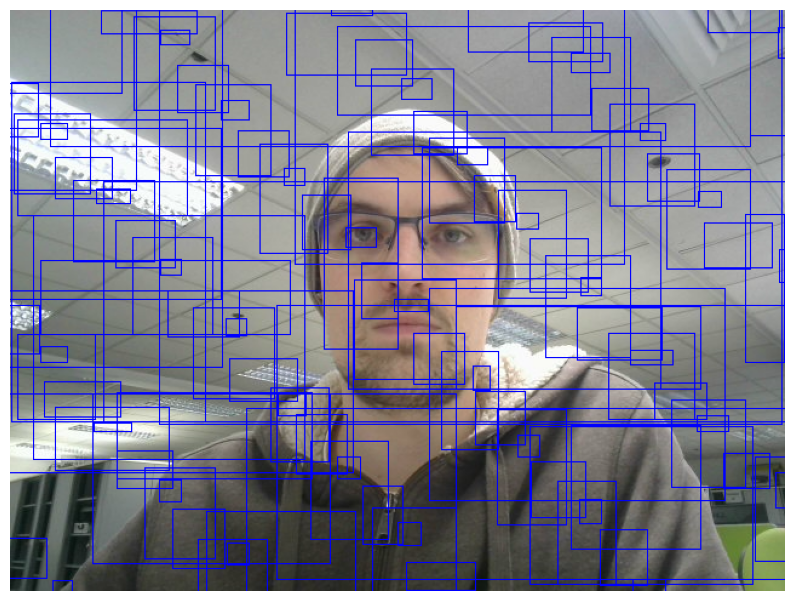
\includegraphics[scale=0.35]{m+m_images/figure4_all_boxes_half_yolo.png}
    \caption{The image after being processed by the YOLO model, showing a significant amount of the bounding boxes predicted by the model, even ones with zero confidence}
    \label{figure:yoloallboxes}
\end{figure}

The YOLO algorithm employs a technique where the input image is partitioned into a grid of cells. Within each cell, YOLO predicts the bounding boxes and class probabilities for objects in that cell. In particular, every grid cell is responsible for predicting several bounding boxes, whether or not objects exist within that cell. This approach ensures that YOLO preserves spatial information and can accurately identify objects of diverse sizes and aspect ratios.

The YOLO model applies a regression approach to anticipate bounding boxes, which are denoted by a series of coordinates for the corresponding grid cell. In addition, the model estimates the confidence score for each bounding box, which signifies the probability of an object being present in the box and the predicted box's accuracy. This score considers both the objectness probability (the probability of an object being present within the bounding box) and the precision of the box's coordinates. YOLO then forecasts class probabilities for each bounding box to recognise the occurrence of specific objects within the image. \cite{Redmon2015-eb}

\begin{figure}[!htb]
    \centering{}
    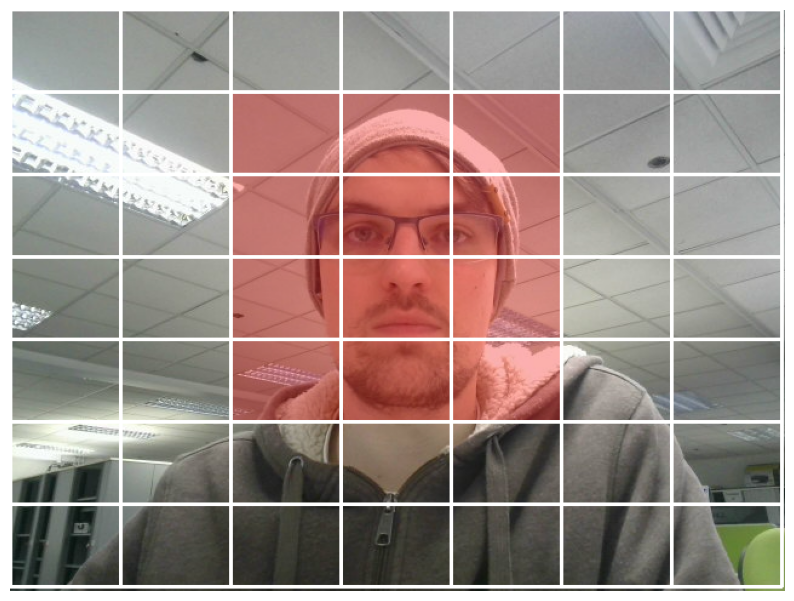
\includegraphics[scale=0.35]{m+m_images/figure2_grid_highlighted_yolo.png}
    \caption{Image showing the grid cells used by the YOLO model to predict confidence scores and bounding boxes, red boxes signifies the grid cells with the highest probability of containing the object}
    \label{figure:yologrid}
\end{figure}
\begin{figure}[!htb]
    \centering{}
    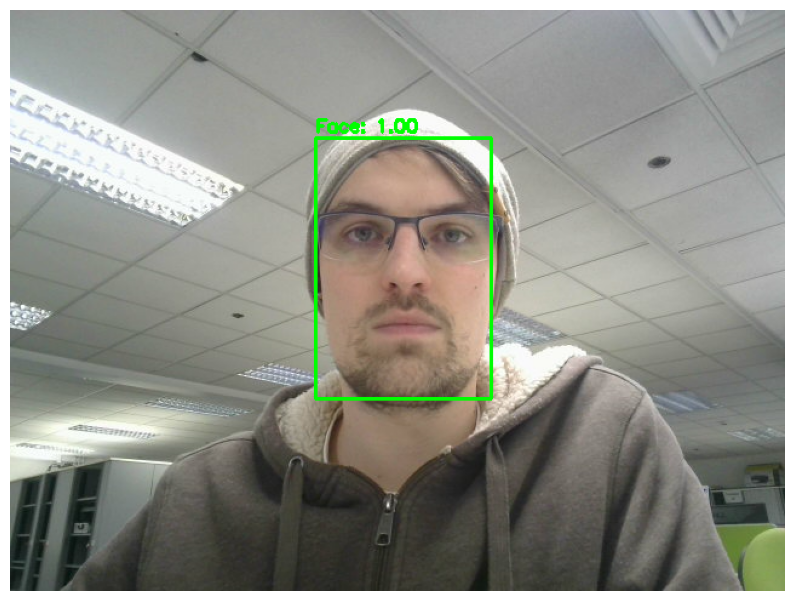
\includegraphics[scale=0.35]{m+m_images/figure3_detection_yolo.png}
    \caption{The image with the final predicted bounding boxes after applying non-maximum suppression}
    \label{figure:yolodection}
\end{figure}

YOLO has a smaller variant called Tiny-YOLO. Although they share the same underlying principles and architecture, there are notable differences between the two in terms of model size, speed, and accuracy.

Tiny YOLO is a condensed version of YOLO that prioritises speed and efficiency. Its streamlined network architecture reduces the number of layers and parameters, resulting in a smaller model size. This makes Tiny YOLO an excellent choice for real-time applications on devices with limited computational resources. While it may sacrifice some accuracy compared to its larger counterpart, Tiny YOLO still delivers competitive performance in object detection tasks. Its balance between speed and accuracy makes it well suited for a robotics application.

\subsubsection{HOG + Linear SVM}

This consists of two components combined to make a method known for its robustness and efficiency in object detection tasks, including face detection.

The Histogram of Oriented Gradients (HOG) is a feature descriptor, it focuses on the structure or shape of an object by capturing the distribution of intensity gradients or edge directions. The first step is gradient computation, typically done using a filter, such as the Sobel operator.

\begin{figure}[!htb]
    \centering{}
    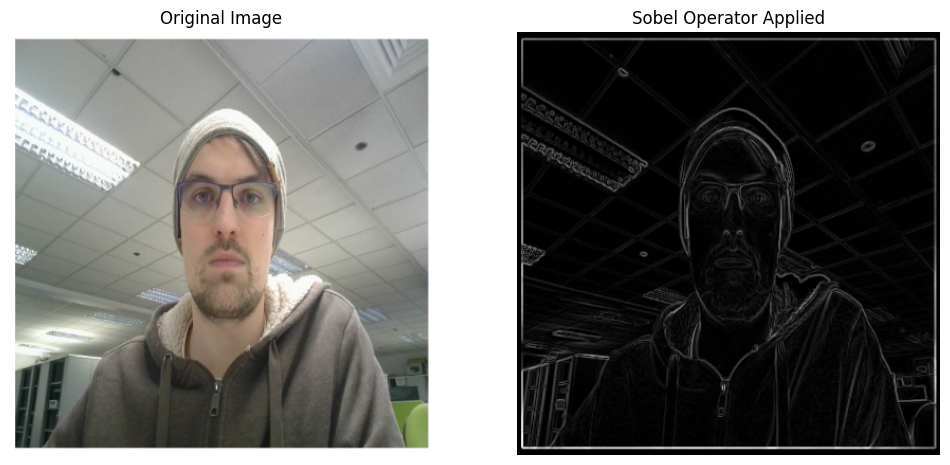
\includegraphics[scale=0.35]{m+m_images/figure1_sobel_hog.png}
    \caption{The resulting image after the Sobel operator}
    \label{figure:hogsobel}
\end{figure}

The image is first divided into small spatial regions called cells, such as 8\(\times\)8 pixels. A histogram of gradient directions is created for each cell, with the magnitude of each gradient used to vote into the histogram bins based on the orientation. Typically, 9 bins are used, covering 0 to 180 degrees.

Histograms are usually normalised to address differences in illumination and contrast. This normalisation involves grouping the cells into larger spatial regions called blocks, for example, 2\(\times\)2 cells to a block. The histograms within a block are then concatenated to form the block descriptor. The normalisation factor is then applied and typically includes options such as L2-norm, L2-Hys, L1-norm, or L1-sqrt.

A detection window is then moved across the image at multiple scales. For each window, a HOG descriptor is calculated and used in the linear SVM.

\begin{figure}[!htb]
    \centering{}
    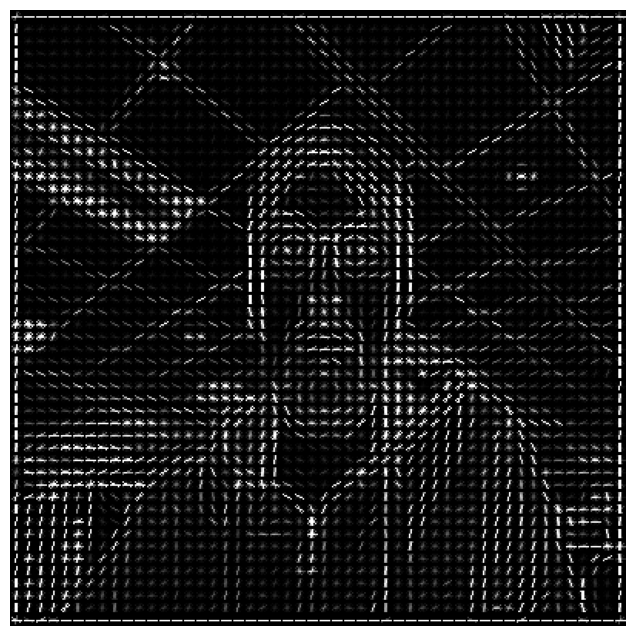
\includegraphics[scale=0.35]{m+m_images/figure2_hog_descriptor_visualised_hog.png}
    \caption{Visualisation of the HOG descriptor}
    \label{figure:hogdescriptor}
\end{figure}

The linear Support Vector Machine (SVM) is a type of supervised learning algorithm specifically designed for binary classification tasks. In the context of face detection, the SVM is used to distinguish between face and non-face HOG descriptors. This involves training the SVM on a dataset containing labelled examples of both faces and non-faces, each represented by its corresponding HOG descriptor. During the detection process, the HOG descriptor of each detection window is computed and then entered into the trained SVM classifier. Based on the input, the SVM generates a score that indicates the likelihood of the window being a face or a non-face. Typically, windows with scores that surpass a certain threshold are classified as faces. \cite{1467360}

\subsection{Emotion Recognition Model}

After successfully detecting faces, an emotion recognition system is created using a Convolutional Neural Network (CNN) implemented in TensorFlow. The CNN model will be taught to categorise facial expressions into specific emotion categories, including happiness, sadness, anger, surprise, fear, and disgust. Using the TensorFlow framework gives a flexible and effective platform for developing, training, and implementing deep learning models.

In summary, the methodology for emotion detection involved testing multiple facial detection algorithms, including YOLOv4, dlib, and Haar Cascade. This will be followed by the implementation of a CNN model in TensorFlow for emotion recognition. This comprehensive approach aims to develop a robust and accurate system for real-time emotion detection from visual inputs.

Three models, VGG16, ResNet50 and MobileNetV2, were tested.

\subsubsection{MobileNetV2, ResNet50, and VGG16}

Convolutional Neural Networks (CNNs) are by far the most widely used architectures in emotion recognition research. Their ability to automatically learn hierarchical feature representations from raw image data makes them highly effective for complex tasks like facial emotion detection. However, despite their popularity, many studies in the literature do not specify the exact CNN architecture used, leaving out important details about model choice and design. This lack of transparency can make it difficult to assess and compare the performance of different approaches across datasets and applications.

The three CNN architectures considered in this work—MobileNetV2, ResNet50, and VGG16—were all used to high degrees of success in the literature. Each offers different trade-offs in terms of accuracy, efficiency, and computational requirements.

MobileNetV2 is a lightweight CNN that uses depthwise separable convolutions to reduce the number of parameters and computations, making it highly efficient for real-time applications on devices with limited resources. Its simplicity makes it ideal for mobile and embedded systems, but this efficiency comes at the cost of potentially missing more complex emotional cues in images.

ResNet50, on the other hand, uses a much deeper network with residual learning to solve the problem of vanishing gradients, allowing it to learn more detailed and hierarchical features. This makes ResNet50 highly effective for recognising subtle facial expressions, although its deep architecture increases computational demand, making it less suitable for real-time systems without powerful hardware.

VGG16, known for its simplicity and effectiveness, uses small convolutional filters (3\(\times\)3) across 16 layers. It is particularly good at capturing fine-grained visual details, but its large number of parameters makes it resource-intensive, resulting in slower processing times compared to more optimised models like MobileNetV2.

\begin{figure}[!htb]
    \centering{}
    \includegraphics[scale=0.15]{m+m_images/VGG16.png}
    \caption{Visualisation of VGG16}
    \label{figure:vggresnetmobilenet}
\end{figure}

In this work, all models were trained using transfer learning, a technique where a pre-trained CNN is fine-tuned on a new dataset. Transfer learning leverages the knowledge these networks have already gained from training on large-scale image datasets, such as ImageNet, to accelerate learning on smaller, domain-specific datasets. This approach significantly reduces computational resources and training time required, while still achieving high accuracy. By reusing learned features from earlier layers and adapting them to emotion recognition, transfer learning allows these models to generalise well, even when trained on limited data specific to facial emotions.

\subsection{Datasets}

\subsubsection{Face Detection Dataset}

The WIDER FACE dataset \cite{yang2016wider} has been meticulously curated to support research in face detection and recognition tasks. It comprises 12,878 images in the training set and 3,224 images in the validation set, sourced from a wide variety of environments. Each image is annotated with one or more bounding boxes that precisely capture the position, orientation and scale of each face, thereby accommodating the extensive variability found in real-world scenarios.

\begin{figure}[!htb]
    \centering{}
    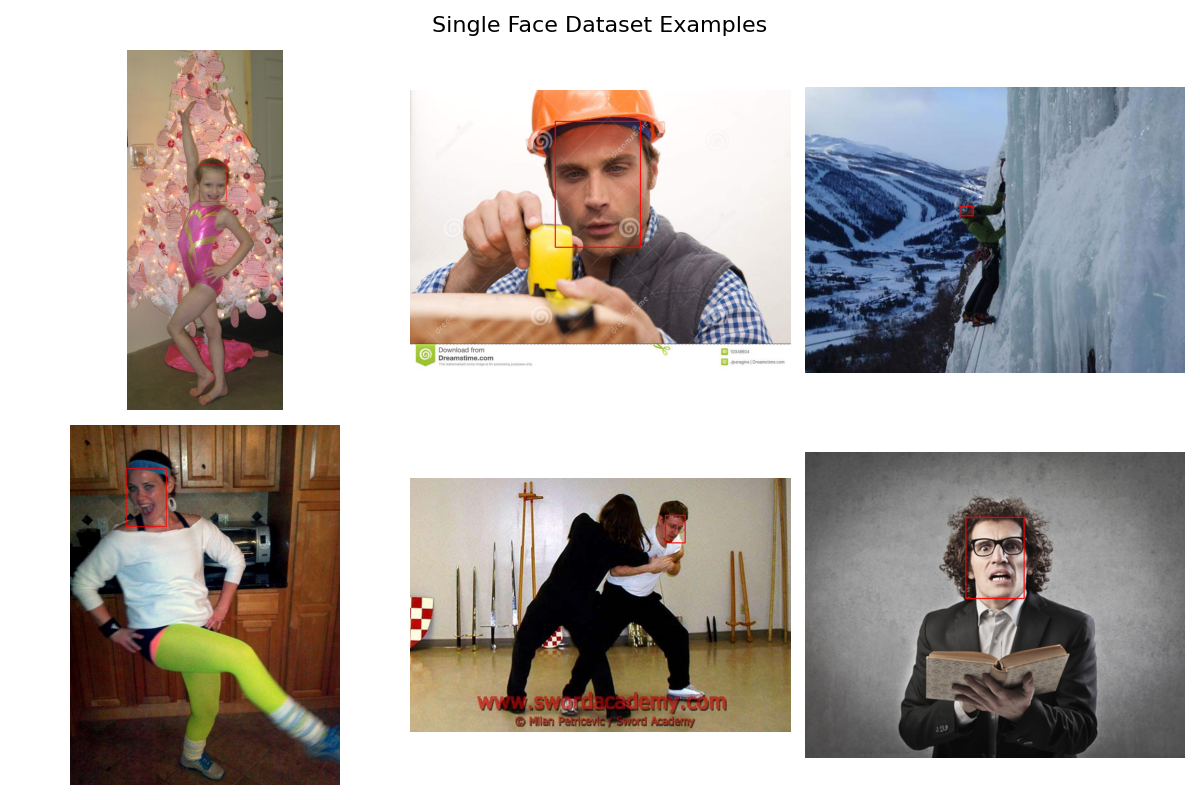
\includegraphics[scale=0.35]{m+m_images/single_face_figure_samples.png}
    \caption{A sample of images from the single-face subset of the WIDER FACE dataset}
    \label{figure:singlefacesamples}
\end{figure}

This dataset is distinguished by its rich diversity in subjects, scenes, and environmental conditions. It features images captured in both indoor and outdoor settings, including crowded environments, street scenes, and surveillance footage. The annotations reflect a broad range of lighting conditions, facial poses, and occlusions, making the dataset highly challenging and suitable for evaluating the robustness of face detection algorithms.

\begin{figure}[!htb]
    \centering{}
    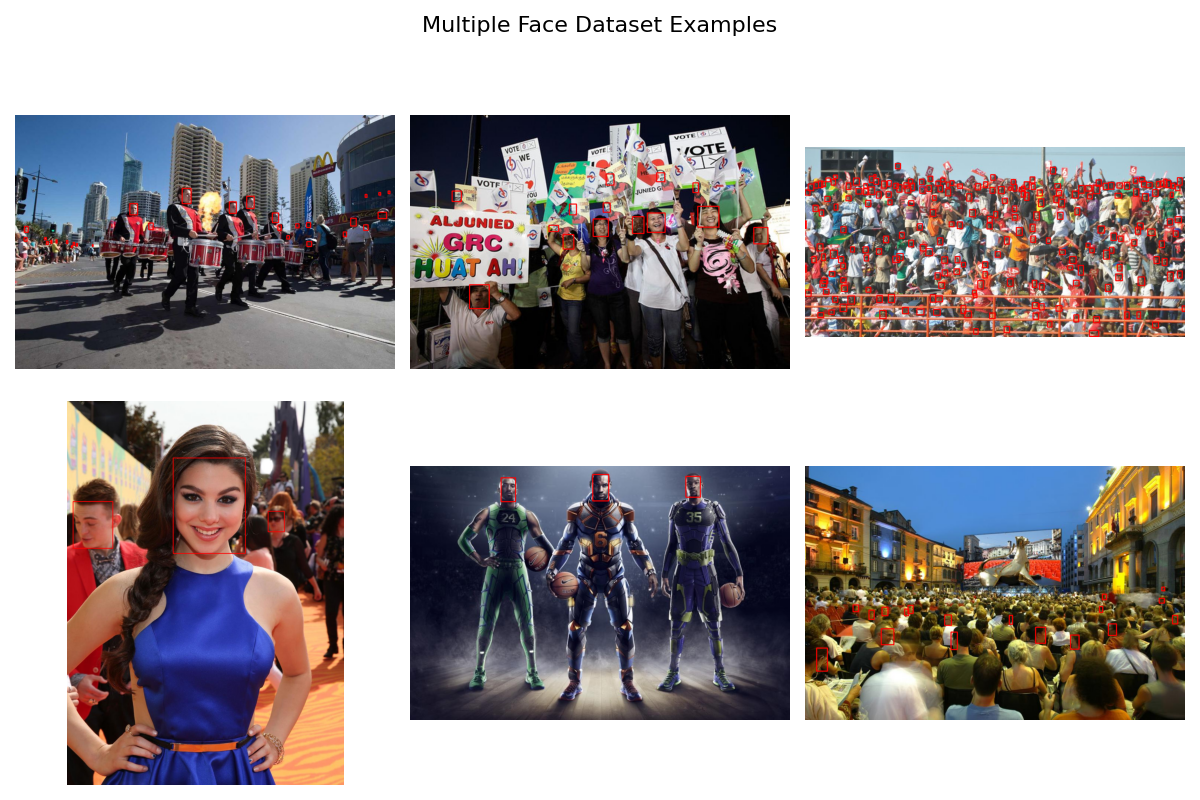
\includegraphics[scale=0.35]{m+m_images/multi_face_figure_samples.png}
    \caption{A sample of images from the multi-face subset of the WIDER FACE dataset}
    \label{figure:multifacesamples}
\end{figure}

For the experiments, the dataset was further subdivided into two distinct evaluation subsets. The first subset consists of images containing only one face per image (1,342 training and 334 validation images), providing a more controlled scenario with minimal distractions. The second subset comprises images with multiple faces (8,245 training and 2,104 validation images), designed to assess the model's performance under more complex conditions with higher face density. Figures \ref{figure:singlefacesamples} and \ref{figure:multifacesamples} illustrate examples from these subsets, highlighting the diversity within the dataset.

\subsubsection{Emotion Recognition Dataset}

The datasets used for training the emotion recognition models were FERPlus \cite{BarsoumICMI2016} and an adapted version of CK+ \cite{5543262}. Both datasets are publicly available and contain images depicting a range of facial expressions in unconstrained environments. Sample images from these datasets are presented in Figure \ref{figure:sample_imgs}.

\begin{figure}[!htb]
    \centering
    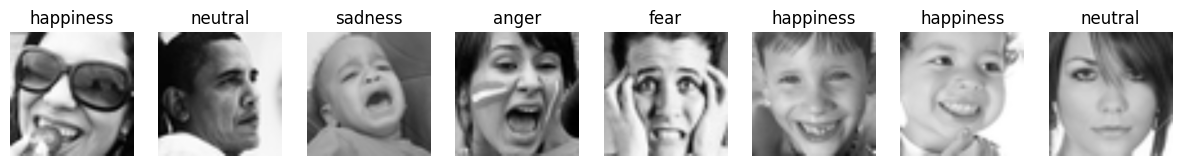
\includegraphics[scale=0.5]{m+m_images/random_imgs.png}
    \caption{Sample of images from the combined FERPlus and CK+ dataset}
    \label{figure:sample_imgs}
\end{figure}

FERPlus is an improved version of the FER2013 dataset, addressing issues such as mislabeled samples and non-face images that previously led to limited recognition accuracy. The dataset was re-annotated using 10 crowd-sourced labelers, categorising each image into one of ten classes: eight emotion categories (happiness, neutral, sadness, surprise, fear, disgust, contempt, and anger) and two additional categories (unknown' for indeterminate emotions and non-face' for images that do not contain a human face). A maximum voting method was used to assign a single label to each image. The dataset consists of 28,386 training images, 3,546 private test images, and 3,553 public test images, with the distribution of emotions detailed in Table \ref{tab:emotion_distribution}.

\begin{table}[!htb]
\centering{}
\caption{Emotion distribution of the training dataset}
\begin{tabular}{|l|c|c|c|c|}
\hline
    \textbf{Emotion}   & \textbf{PrivateTest} & \textbf{PublicTest} & \textbf{Training} & \textbf{Total} \\ \hline
    \textbf{Anger}     & 325                  & 319                 & 2,466             & 3,110          \\ \hline
    \textbf{Contempt}  & 27                   & 24                  & 165               & 216            \\ \hline
    \textbf{Disgust}   & 23                   & 34                  & 191               & 248            \\ \hline
    \textbf{Fear}      & 93                   & 74                  & 652               & 819            \\ \hline
    \textbf{Happiness} & 928                  & 899                 & 7,528             & 9,355          \\ \hline
    \textbf{Neutral}   & 1,262                & 1,335               & 10,308            & 12,905         \\ \hline
    \textbf{Sadness}   & 444                  & 412                 & 3,514             & 4,370          \\ \hline
    \textbf{Surprise}  & 444                  & 456                 & 3,562             & 4,462          \\ \hline
    \textbf{Total}     & 3,546                & 3,553               & 28,386            & 35,485         \\ \hline
\end{tabular}
\label{tab:emotion_distribution}
\end{table}

The Extended Cohn-Kanade (CK+) dataset consists of 593 video sequences from 123 subjects aged 18 to 50 years. The dataset includes individuals of diverse gender and ethnicity backgrounds, with 69\% female, 81\% Euro-American, 13\% Afro-American, and 6\% from other groups. Each sequence progresses from a neutral facial expression to a peak expression, recorded at 30 frames per second at a resolution of 640\(\times\)480 pixels. The dataset includes seven labeled emotions: anger, contempt, disgust, fear, happiness, sadness, and surprise.

\begin{table}[!htb]
    \centering{}
    \caption{Image counts for each emotion in CK+}
    \begin{tabular}{|l|c|}
        \hline
        \textbf{Emotion}   & \textbf{Count} \\ \hline
        \textbf{Anger}     & 135   \\ \hline
        \textbf{Contempt}  & 54    \\ \hline
        \textbf{Disgust}   & 177   \\ \hline
        \textbf{Fear}      & 75    \\ \hline
        \textbf{Happiness} & 207   \\ \hline
        \textbf{Sadness}   & 84    \\ \hline
        \textbf{Surprise}  & 249   \\ \hline
    \end{tabular}
\label{tab:emotion_counts_ck+}
\end{table}

For consistency with FERPlus, an altered version of CK+ was used, where frames were preprocessed to be grayscale and resized to 48\(\times\)48 pixels. The adapted dataset was retrieved from the database sharing website Kaggle and included the following modifications:

\begin{itemize}
    \item{} Contains adapted data up to 920 images from 920 original CK+ dataset
    \item{} Data is already reshaped to 48\(\times\)48 pixels, in grayscale format and facecropped using haarcascade\_frontalface\_default.
    \item{} Noisy (based on room light/hair format/skin colour) images were adapted to be clearly identified using Haar classifier.
    \item{} Columns from file are defined as emotion/pixels/Usage
\end{itemize}

The final dataset contains the emotion distribution summarised in Table \ref{tab:emotion_counts_ck+}.


The Expressions in the Wild (ExpW) dataset was used to evaluate the performance of the emotion recognition system. ExpW consists of 106,962 images, almost all (91,793) are annotated facial images collected from the web, covering a diverse range of real-world conditions such as varying lighting, occlusions, and head poses. Each image is labeled with one of seven emotion categories: neutral, happiness, sadness, surprise, fear, disgust, and anger. ExpW contains highly unconstrained facial expressions, making it a valuable benchmark for testing the robustness of the trained model in real-world scenarios.

\begin{figure}[!htb]
    \centering{}
    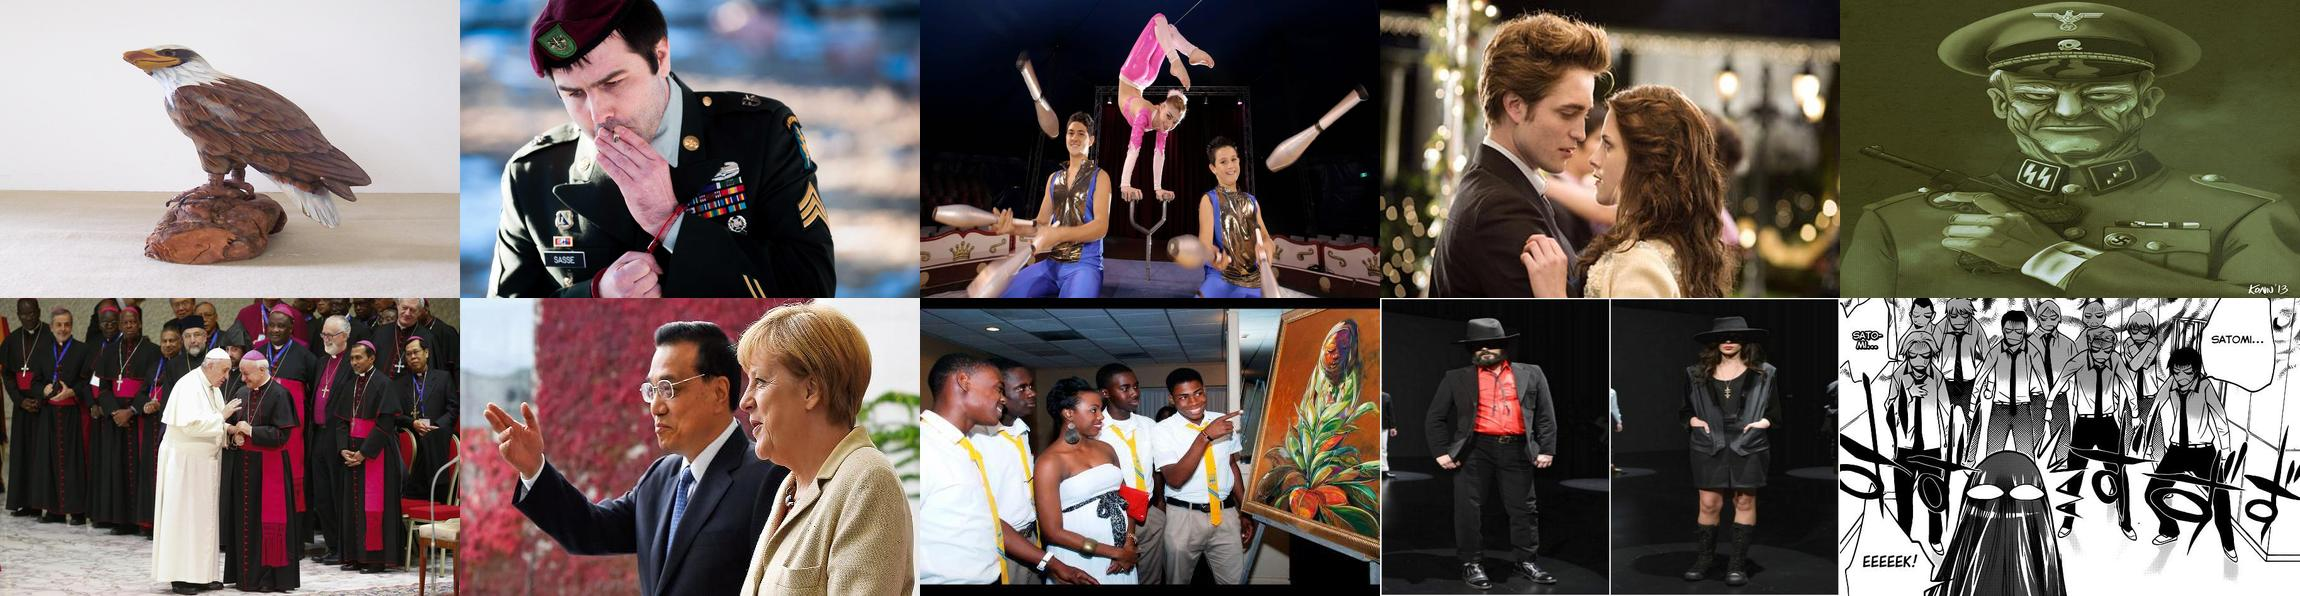
\includegraphics[scale=0.18]{m+m_images/exp_w_sample.jpg}
    \caption{A random selection of images from the ExpW dataset}
    \label{figure:exp_w_sample}
\end{figure}

A selection of random images from ExpW can be seen in \ref{figure:exp_w_sample}.


